\section{A type system for determinism}\label{design}

This section presents the key aspects of the design of our type system,
called \ourTypeSystem, in the context of a core calculus for an
object-oriented language.


\subsection{Preliminaries}

%% This section is too basic, and therefore is boring because most readers
%% will already know it.  It also delays the interesting parts of the paper
%% for too long.  We can introduce concepts as they are needed in the rest
%% of the paper.
% \subsection{Type checking background}\label{type-checking}
% The major components of a type system include: 1) \textit{types}, 2) \textit{subtyping rules}, and 3) \textit{dataflow analysis}.
% A \textit{type} serves as an abstraction for the set of acceptable values for any expression. The types in a type system form a lattice of finite height. 
% The hierarchy of types in this lattice defines subtyping relationships among them.
% In our framework, we require every type hierarchy to define a unique\<@Top> and a \<@Bottom> element. This ensures that
% any given pair of types has a \textit{least upper bound} and a \textit{greatest lower bound}.
% Throughout this paper, we use the notation \<@A> <: \<@B> to denote that type \<@A> is a subtype of type \<@B>.
% As an illustration of the type hierarchy, consider the lattice of types shown in \cref{fig-example-lattice}.
% \begin{figure}
%     \begin{center}
%         \includegraphics[scale=0.15]{lattice}
%     \end{center}
%     \caption{Example type hierarchy}
%     \label{fig-example-lattice}
% \end{figure}
% In this type system, \<@C> is a subtype of \<@A> as well as \<@B> and types \<@A> and \<@B> are incomparable.
% The type checker now performs additional type checking (similar to javac's type checking) with respect to this type hierarchy
% and reports any violations. The snippet in \cref{code-invalid1} would result in an error at the assignment statements:
% \begin{figure}
%     \begin{verbatim}
%     @A int x; @B int y; @C int z;
%     x = y;    // Because types @A and @B are incomparable.
%     z = x;    // Because @C is a subtype of @A.
%     \end{verbatim}
% \caption{Example: Invalid assingment}
% \label{code-invalid1}
% \end{figure}
% 
% %Method overriding and example
% For method overriding, the usual rules apply for parameters and arguments i.e covariant subtyping for parameters
% and contravariant subtyping for return types. Consider the example in \cref{code-invalid2} where method \<foo> of \<class X> is overridden
% in \<class Y>.
% \begin{figure}
%     \begin{verbatim}
%     class X {
%         @B int foo(@C int param) {}
%     }
%     class Y extends X {
%         @C int foo(@B int param) {}
%     }
%     \end{verbatim}
%     \caption{Example: Invalid Method override}
%     \label{code-invalid2}
% \end{figure}
% 
% The overriding method is invalid for two reasons: type of the parameter (\<@B>) is not a subtype of the parameter type in the overridden method (\<@C>) and the return type (\<@C>) is not a supertype of the return type of the overridden method (\<@B>).
% 
% %collections type parameters - invariant
% Collection types are invariant. So, if a \<List> x is declared as \codeid{@A List<@A String> x;} and another \<List y> is declared
% as  \codeid{@A List<@B String> y;}, writing \<x = y> would result in an error.
% 
% %covariant array types
% Arrays follow covariant subtyping rules in java. Therefore, the assignment statement \<@A int @A[] x = y;> where \<y> was 
% declared as \<@B int @A[] y> would type check without any warning.



%\todo{Need some background around here about what a type qualifier is,
%  how it is represented in Java, and how to read a type \<@Q BaseType>.}

\todo{Greek letters go after this paragraph.}

In a type system,
a \textit{type} represents a set of values.  It abstracts or restricts the
set of possible run-time values that an expression may evaluate to.
A programming language provides \emph{basetypes}, such as \<int>.
A \textit{type qualifier} on a basetype adds additional constraints;
that is, it reduces the size of the set of values.
An example type qualifier is \<Positive>,\todo{should all type qualifiers
  be lowercase in this section??} and a type (which combines a qualifier
anda basetype) is \<Positive int>.
A polymorphic type such as \<List> can be instantiated by a type argument,
as in \ptype{List}{Positive int}.

A type checker verifies the types written in a program.

\begin{figure}
    \bigskip

    $\infer{\tau_1 \sqsubseteq \tau_3}{\tau_1 \sqsubseteq \tau_2 \quad \tau_2 \sqsubseteq \tau_3}
    \quad\quad
    \infer[\textsc{subtyping}]{\Gamma \vdash x : \tau_2}{\Gamma \vdash x : \tau_1 & \tau_1 \sqsubseteq \tau_2}$
    
    \bigskip
    
    $\infer[\textsc{method call}]{\|method|(\overline{a_i}) : \tau_r}{\tau_r \  \|method|(\overline{\tau_i \  p_i}) & \overline{a_i : \tau_i}}$
    
    \bigskip
    
    $\infer[\textsc{invariant type param}]{C_1\angles{\overline{\tau_i}}
      \sqsubseteq C_2\angles{\overline{\tau_i}}}{C_1 \sqsubseteq C_2}$
    
    \caption{A sampling of standard type checking rules.  Most standard rules are omitted
    for brevity.  $\sqsubseteq$ is overloaded for classes and types.}
    \label{typecheck-rules-standard}
\end{figure}

\begin{figure}
    \bigskip

    $\infer{\Det \sqsubseteq \OrderNonDet}{}
    \quad\quad
    \infer{\OrderNonDet \sqsubseteq \NonDet}{}$
    
    \bigskip

    $\infer{\kappa_1 \beta \sqsubseteq \kappa_2 \beta}{\kappa_1 \sqsubseteq \kappa_2}
    \quad\quad
    \infer{\kappa \beta_1 \sqsubseteq \kappa \beta_2}{\beta_1 \sqsubseteq \beta_2}$
    
    
    \caption{Type checking rules.  $\sqsubseteq$ is overloaded for classes,
    basetypes, type qualifiers, and types.}
    \label{fig:typecheck-rules}
\end{figure}


\subsection{Determinism types}\label{type-hierarchy}

\begin{wrapfigure}{R}{0.3\textwidth}
    \begin{center}
        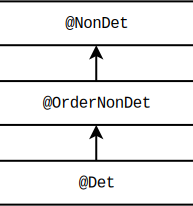
\includegraphics[scale=0.5]{determinism}
    \end{center}
    \caption{Determinism type qualifier hierarchy}
    \label{fig:determinism-hierarchy}
\todo{Drop the at-signs (@).  The text is weirdly small for the box.
  Probably just redraw this.}
\end{wrapfigure}

The core of the determinism type system is the following type qualifiers:
%\todo{introduce just @Det and @NonDet first, and then @OrderNonDet after polymorphism.}
\begin{itemize}
    \item \<NonDet> indicates
    that the expression might have different values in two different executions.
    \item \<OrderNonDet> indicates that the expression is a collection or
      map that contains the same elements in every execution, but possibly
      in a different order.
    \item \<Det> indicates that
    the expression evaluates to the same value (with respect to \<.equals()>) in all
    executions; for a collection, iteration also yields the values in the same
    order.
\end{itemize}
\Cref{fig:typecheck-rules,fig:determinism-hierarchy} show their subtyping relationship.

\<OrderNonDet> may only be written on collections and maps.  Our implementation
handles array types, and any class (including user-defined classes) that
implements the \<Iterable> or \<Iterator> interfaces; this includes all
Java collections such as \<List>s and \<Set>s.  For simplicity, and because
the semantics and rules are similar even though the syntax varies, this
paper uses the term ``collection'' and the type \<Collection> to represent
all these types.

A map is a dictionary or associative array, such as a hash table.
Our type system largely treats a map as a collection of key--value pairs.  Like a
collection, a map may be \<Det>, \<OrderNonDet>, or \<NonDet>.  (In Java,
\<HashMap> cannot be deterministic, but \<TreeMap> and \<LinkedHashMap>
can.\todo{forward reference?})


In \cref{code-determinism}, we present some of the JDK methods that we have annotated with our determinism types and give examples of
client code that would produce errors at compile time.
\begin{figure}
    \begin{verbatim}
    // Annotated JDK methods
    public class Random implements java.io.Serializable {
        public @NonDet Random() {}
    }
    public class PrintStream extends FilterOutputStream 
        implements Appendable, Closeable {
        public void println(@Det Object x) {}
    }
    
    // Client code
    class Client {
        void test() {
            @Det double d = Math.random(); // Error - subtyping rules violated.
            @NonDet double nd = Math.random(); // No error.
            System.out.println(nd); // Error - println takes @Det arguments.
        }
    }
    \end{verbatim}
    \caption{Example: Errors detected by \theDeterminismChecker.}
\todo{Use real examples of bugs from case studies, throughout.  Artificial
  examples are less compelling (and lead the reader to wonder whether no
  real example exist).  Put the first example of an error in a figure in
  Section 1, to help with motivating the problem.}
    \label{code-determinism}
\end{figure}


\subsection{Collection types}\label{collection-rules}

\todo{Note that the \textsc{ordernondet} versions also handle \<Det>,
  because $\<Det> \sqsubseteq \<OrderNonDet>$.}

\begin{figure}
    $\infer[\textsc{any type}]{\wellformed{\kappa \  \beta}}{\kappa : \|Det / NonDet|}$
    
    \bigskip
    
    $\infer[\textsc{ordernondet collection}]{\wellformed{\kappa_c \  \beta_c \angles{\kappa_e \ \beta_e}}}{\kappa_c : \|OrderNonDet/Det| & \kappa_e \sqsubseteq \kappa_c & \beta_c \sqsubseteq \<Collection>}$
    
    \bigskip
    
    $\infer[\textsc{nondet collection}]{\wellformed{\|NonDet| \ \beta_c\angles{\|NonDet| \ \beta_e}}}{\beta_c \sqsubseteq \<Collection>}$
    
    \bigskip
    
%      $\infer[\textsc{ordernondet array}]{\wellformed{\kappa_e \ \beta_e \ \  \kappa_a []}}{\kappa_a : \|OrderNonDet/Det| & \kappa_e \sqsubseteq \kappa_a }$
%     
%     \bigskip
%     
%     $\infer[\textsc{nondet array}]{\wellformed{\|NonDet| \ \beta_e \ \  \|NonDet| []}}{}$
%     
%     \bigskip
    
    $\infer[\textsc{ordernondet map}]{\wellformed{\kappa_m \  \beta_m \angles{\kappa_k \ \beta_k, \kappa_v \ \beta_v}}}{\kappa_m: \|OrderNonDet/Det| & \kappa_k \sqsubseteq \kappa_m & \kappa_v \sqsubseteq \kappa_m & \beta_m \sqsubseteq \<Map>}$
    
    \bigskip
    
    $\infer[\textsc{nondet map}]{\wellformed{\|NonDet| \ \beta_m\angles{\|NonDet| \ \beta_k, \|NonDet| \ \beta_v}}}{\beta_m \sqsubseteq \<Map>}$
    
    \caption{Type well formedness}
\todo{The \textsc{any type} rule is not correct, because not every type is
  well-formed.  It needs an antecedent stating that $\beta$ is not a
  collection or map.}

\todo{The collection rules do not permit nested collections; similarly, the
  (currently commented out) array rules did not permit any two-dimensional
  array to be well-formed.  There is a bigger issue here.
  Consider the ``nondet collection'' rule.  $\beta_c$ is a class (we need
  to use a different symbol for it, probably $c$), but $\beta_e$ should be
  a full type, which might contain type qualifiers within it.  (Actually,
  $\|NonDet|\ \beta_e$ is a type, not $\beta_e$ itself.)  So, there should
  be an antecedent stating that $\|NonDet| \beta_e$ is well-formed, and
  for the ``ordernondet collection'' rule stating that $\kappa_e \beta_e$
  is well-formed.  Likewise, antecedents are needed for the map rules.
  Otherwise, these rules permit construction of $\<Map>\angles{\tau'}$
  where $\tau'$ is itself not well-defined.}

\todo{``$\kappa : \|Det / NonDet|$'' should be ``$\kappa = \|Det /
  NonDet|$'' or (better)
  ``$\kappa \in \{\|Det|, \|NonDet|\}$''.
  You could also express $\kappa_c : \|OrderNonDet/Det|$ as just
  $\kappa_c \sqsubseteq \|OrderNonDet|$ since $\|Det| \sqsubseteq \|OrderNonDet|$.
}

  \label{type-validity}
\end{figure}

\Cref{type-validity} shows the type validity\todo{The caption says
  ``type well formedness''.  Choose one term and use it consistently
  throughout.}
rules of our type system. A type $\tau$ is represented as $\kappa \ \beta$
where $\kappa$ is a type qualifier (that is, \<NonDet>, \<OrderNonDet>, or
\<Det>) and $\beta$ is a Java basetype.
As stated in the rule $\textsc{any type}$, the types \<Det> and \<NonDet>
can be written on any Java basetype.\todo{As noted in figure caption, that's
  not true, in some contexts such as a type argument.}

The determinism type qualifier on a collection must be a supertype or equal to
its element type qualifier (Rule $\textsc{ordernondet collection}$ in \cref{fig-determinism-collections}).
If the Collection is \<NonDet>, then the type argument may not be
\<Det> or \<OrderNonDet> (Rule $\textsc{nondet collection}$ in \cref{type-validity}). Although such types could exist, they are
disallowed to prevent the following bug:

\begin{verbatim}
public static void add(@NonDet List<@Det String> list, @NonDet int index, @Det String s) {
    list.add(index, s);
}

public static void f(@Det List<@Det String> list, @NonDet int index, @Det String s) {
    add(list, index, s);
}
\end{verbatim}

The possibility of mutation allows us to add to the \<Det List> at a
\<NonDet> index, which is unsound.

\todo{Some notes:}
Typical type for \<get> is \\
$\forall \tau . \<List>\angles{\tau} \times \<int> \rightarrow \tau$ \\
but we need to change that.  If either argument is \<OrderNonDet> or \<NonDet>, then the
result is \<NonDet>.
If both arguments are \<Det>, the result is $\tau$ as usual.
\todo{In that case, we know that $\tau = \<Det> \beta$.}



\smallskip
\noindent
\begin{minipage}{.48\textwidth}
Some examples of valid types are:
% Using "~" instead of "\ " does not work within \codeid :-(
\begin{smaller}
\begin{Verbatim}
@NonDet      List<@NonDet      Integer>
@OrderNonDet List<@OrderNonDet Set<...>>
@OrderNonDet List<@Det         Integer>
@Det         List<@Det         Integer>

\end{Verbatim}
\end{smaller}
\end{minipage}
\hfill
\begin{minipage}{.46\textwidth}
These types are invalid:
\begin{smaller}
\begin{Verbatim}
@NonDet      List<@OrderNonDet Set<...>>
@NonDet      List<@Det         Integer>
@OrderNonDet List<@NonDet      Integer>
@Det         List<@NonDet      Integer>
@Det         List<@OrderNonDet Set<...>>
\end{Verbatim}
\end{smaller}
\end{minipage}
\smallskip

\begin{figure}
    \centering
    \begin{tabular}{|l|l|l|l|l|}
        \cline{3-5}
        \multicolumn{2}{c|}{~}  &  \multicolumn{3}{c|}{element type} \\ \cline{3-5}
        \multicolumn{2}{c|}{~}  & NonDet     & OrderNonDet & Det \\ \hline
        & NonDet      &   valid    &  invalid    & invalid  \\ \cline{2-5}
        Collection    & OrderNonDet &   invalid  &  valid      & valid  \\ \cline{2-5}
        & Det         &   invalid  &  invalid    & valid      \\ \hline
    \end{tabular}
    \caption{Valid Collection declarations.  The Collection's type qualifier
        must be a supertype or equal to the element type.}
    \label{fig-determinism-collections}
\end{figure}

A collection or map annotated as \<OrderNonDet> has the following properties:
\todo{Write these as type rules.}
\begin{enumerate}
    \item The individual elements extracted by iterating over the collection get the type \<NonDet>.
    \item Accessing properties such as \<size()> or querying if the collection \<isEmpty()> will return types
    that are annotated as \<Det> as they do not depend on the iteration order. 
\end{enumerate}



\subsection{Polymorphism}\label{polymorphism}

Our type system supports three types of polymorphism:  type
polymorphism, basetype polymorphism, and qualifier polymorphism.
\todo{Give an example for each.}
\begin{itemize}
\item
In \theDeterminismCheckerImplementation,
type polymorphism is handled by Java's generics mechanism, which
\theDeterminismChecker fully supports, including class and method generics,
inference, etc.
Given the Java declaration
\begin{Verbatim}
<T> T identity(T arg) { return arg; }
\end{Verbatim}
the type of \<identity(arg)> is the same as the type of
\<arg>, and a programmer can write a type such as \codeid{List<@NonDet
  Integer>} (but see below for details about collections).
\item
Basetype polymorphism is enabled by writing a type qualifier on a use of a
type variable, which overrides the type qualifier at the instantiation
site.
For example, a \<choose> operation on sets could be defined in Java as
\begin{Verbatim}
class ChooseableSet<T> implements Set<T> {
  // return an arbitrary element from the set
  @NonDet T choose();
}
\end{Verbatim}
\item
Java does not provide a syntax that can be used for qualifier polymorphism,
so we use a special type qualifier name, \<@PolyDet>.
A qualifier-polymorphic method \<m> with signature $\forall \kappa . \kappa\ \<int> \times \<Det boolean> \rightarrow
\kappa\ \<String>$ would be written in our dialect of Java as
\begin{Verbatim}
@PolyDet String m(@PolyDet int, @Det boolean)
\end{Verbatim}
Each use of \<@PolyDet> stands for a use of the qualifier variable
$\kappa$, and there is no need to declare the qualifier variable $\kappa$.
\TheDeterminismChecker currently supports
qualifier
polymorphism on methods but not on classes.
Therefore, \<@PolyDet> may be written in methods (signatures and bodies)
but not on fields.
\end{itemize}




When a user writes a polymorphic qualifier on a method signature or a type parameter,
it indicates that it could resolve\todo{Should all occurrences of ``resolve'' be ``can be instantiated''} to any type in the type system depending on how it is used.
In \theDeterminismChecker, we define a polymorphic qualifier \<PolyDet>.
One of the most common locations for a polymorphic qualifier is at a method signature.
Consider the following declaration of addition:
\begin{verbatim}
@PolyDet int plus(@PolyDet int a, @PolyDet int b) { return a+b; }
\end{verbatim}
\todo{It has the standard meaning.  There are two ways to interpret this.}
There are two valid instantiations for this declaration:
\begin{enumerate}
    \item @NonDet int plus(@NonDet int a, @NonDet int b) { return a+b; }
    \item @Det int plus(@Det int a, @Det int b) { return a+b; }
\end{enumerate}
This indicates that method \<foo> can be called with arguments having any of the \codeid{Det or NonDet} type qualifiers.
%   (\<@OrderNonDet> is not allowed because it is invalid on primitive types).
 \<PolyDet> resolves to the least upper bound of
the actual types on arguments. For instance, if this method is called as \codeid{foo(@Det String arg1, @NonDet boolean arg2)}, \theDeterminismChecker resolves the method declaration as \codeid{@NonDet int foo(@NonDet String param1, @NonDet boolean param2)}
causing the return type to have the type qualifier \<NonDet>.

\subsection{Polymorphism rules for collections}\label{polymorphism-up-down}

Some types are invalid and must not be permitted (during polymorphic instantiation).

Recall that \theDeterminismChecker does not permit \<OrderNonDet> on a type
that isn't a collection.
As a consequence, resolution of polymorphic type qualifiers at method signatures could have undesirable effects.
Suppose a method declaration is annotated as \codeid{PolyDet int size(PolyDet List<T> list)}. Invoking this method
with an argument of type \codeid{OrderNonDet List<Det String>} will result in \<PolyDet> getting resolved to \<OrderNonDet> which is invalid
on the return type \<int>. We circumvent this scenario by introducing two variants to the \<PolyDet> qualifier, \PolyDetUp
and \PolyDetDown. 

% Not true: We allow Poly(up) and down at every location where Poly is allowed.
%Valid locations for \codeid{@PolyDet("up")} and  \codeid{@PolyDet("down")}:
%$\infer{\wellformed{\kappa \  \beta}}{isParam(\beta) / isReturn(\beta) & \kappa : @PolyDet("up") / @PolyDet("down")}$
%
%Resolution of \<@PolyDet("up")>:\todo{typesetting}
%
%$\infer{\Gamma \vdash x : @NonDet \ \beta_a}{\Gamma \vdash x : \kappa_a \ \beta_a &  \kappa_a : @OrderNonDet/@NonDet & \kappa_p : @PolyDet("up") & \kappa_p \ \beta_p : declaration \ type & \kappa_a \ \beta_a : resolved \ type}$
%
%Resolution of \<@PolyDet("down")>:
%
%$\infer{\Gamma \vdash x : @Det \  \beta_a}{\Gamma \vdash x :  \kappa_a \beta_a & \kappa_a : @OrderNonDet/@Det & \kappa_p : @PolyDet("down") & \kappa_p \ \beta_p : declaration \ type & \kappa_a \ \beta_a : resolved \ type}$

The semantics of these variants are as follows:
\begin{itemize}
    \item \PolyDetUp: Same as \<PolyDet> except when it resolves to \<OrderNonDet>, it is replaced with \<NonDet>.
    \item \PolyDetDown: Same as \<PolyDet> except when it resolves to \<OrderNonDet>, it is replaced with \<Det>.
\end{itemize} 
The modifiers $\uparrow$ and $\downarrow$ are indicative of the subtyping relationship of \<OrderNonDet> with \<NonDet> and \<Det> respectively
in the determinism type hierarchy.

\Cref{fig-poly-resolution} presents the rule for type checking of methods annotated with \<PolyDet> or its variants.
A polymorphic method type checks if every instantiation of \<PolyDet> type checks. If this method has \<PolyDet>$\uparrow$ or \<PolyDet>$\downarrow$
in its signature then the instantiation of \<PolyDet> at that location gets replaced by the appropriate type as shown in Table~\ref{tab-poly-resolutions}.

Annotating \<size()> as \codeid{PolyDet$\downarrow$ int size(PolyDet List<T> list)} will only allow the following type resolutions:
\begin{itemize}
    \item \codeid{@Det int size(@Det List<T> list)}
    \item \codeid{@Det int size(@OrderNonDet List<T> list)}
    \item \codeid{@NonDet int size(@NonDet List<T> list)}
\end{itemize}

\begin{figure}
    $\infer[\textsc{poly resolution}]{\pi_r \ \beta_r\ \<m>(\overline{\pi_i \ \beta_i})\{\ \}}{\forall \kappa \in \{\|NonDet, OrderNonDet, Det|\} : \kappa \ \beta_r\ \<m>(\overline{K \ \beta_i})\{\ \} & \pi_r, \pi_i \in \{\|PolyDet|, \|PolyDet|\uparrow, \|PolyDet|\downarrow    \}}$
    \caption{Polymorphic resolution rule}
    \todo{I'm not sure what this is doing.  What code does it reject?}
    \todo{This suggests that \PolyDetUp is a qualifier, rather than
      $\uparrow$ being an operator on qualifiers.  We should clarify which
      it is.}
    \label{fig-poly-resolution}
\end{figure}

\begin{table}[]
    \begin{tabular}{|l|l|l|}
        \hline
        \textbf{\<PolyDet>} & \textbf{\PolyDetUp} & \textbf{\PolyDetDown} \\ \hline
        \<NonDet> & \<NonDet> &  \<NonDet>\\ \hline
        \<OrderNonDet> & \<NonDet> &  \<Det>\\ \hline
        \<Det> & \<Det> &  \<Det>\\ \hline
    \end{tabular}
\caption{Polymorphic resolution}
\todo{Write this as a rule rather than a table.}
\label{tab-poly-resolutions}
\end{table}

\subsubsection{Differentiating binding and use}\label{bindings-uses}

In order to provide soundness guarantees, we must ensure that a collection that is
declared as \<Det> is not side-effected in non-deterministic ways. Consider the following qualifier 
on the List add method: \codeid{public void add(PolyDet ArrayList<E> this, PolyDet int index, E element)}.
Suppose a client calls this method as follows:
\begin{verbatim}
@Det ArrayList<@Det String> list;
@NonDet int random;
@Det String str;
list.add(random, str);
\end{verbatim}
This will result in the instantiation \codeid{public void add(@NonDet ArrayList<E> this, @NonDet int index, E element)} and
the method invocation will type check. This is problematic because even though \<list> was declared to be \<Det>,
the type checker allows the addition of an element at a \<NonDet> location violating our determinism guarantees.
We prevent this behavior by introducing another variant of \<PolyDet>, \<PolyDet("use")> that does not affect
type instantiations. This is especially useful in preventing methods from non-deterministically modifying the state
of a deterministic receiver. To have this effect, the library method \<ArrayList.add> is annotated as:
\codeid{public void add(PolyDet ArrayList<E> this, PolyDet("use") int index, E element)}.
Since \<PolyDet("use")> has no effect on type instantiations, calling this method on a \<Det List>
will result in the method declaration being resolved as \codeid{public void add(@Det ArrayList<E> this, @Det int index, E element)}
irrespective of the type of \<index>, thereby preventing undesired side-effects.

\subsection{Discussion on defaulting rules}\label{defaulting}

\TheDeterminismChecker applies a default qualifier at each unannotated type
use (except uses of type variables, which already stand for a type that was
defaulted at the instantiation site).
This does not change the expressivity of the type system; it merely makes
the system more convenient to use.

In \theDeterminismChecker, we chose \<PolyDet> as the default for all 
method parameters and return types including constructors.
The rationale for this design choice was to not make our type checker too restrictive by making everything \<Det>.  This implies that
\theDeterminismChecker still allows some non-determinism as long as it doesn't break any determinism specifications explicitly written by the programmer.

\begin{verbatim}
@PolyDet int foo(@PolyDet int x) { ... }

void bar(@NonDet int random, @Det int value) {
    @NonDet int x = foo(random);      // No error.
    @Det int y = foo(value);          // No error.
    System.out.println(foo(random));  // Error.
}
\end{verbatim}
In the example above, the method \codeid{foo} is annotated with the \<PolyDet> type qualifier which allows
the caller method \codeid{bar} to invoke it with both \<Det> and \<NonDet> arguments. \TheDeterminismChecker flags an error 
only when the returned value is used in a way that breaks any deterministic specification (Printing a \<NonDet> value
breaks our determinism guarantees).

\subsection{Dataflow analysis and type refinement}\label{dataflow}
\TheDeterminismChecker performs automatic type inference for local types within method bodies.
It also performs dataflow analysis and refines the types of these locals, thereby reducing the qualifier burden 
on the programmer. Consider the example below:
\begin{verbatim}
void foo(@Det int x) {
    @NonDet int y = x;    // Type of y gets refined to @Det.
    @Det int z = y;       //  No error here.
}
\end{verbatim}
In the example above, even though the local variable \codeid{y} was declared to be \codeid{NonDet}, it gets
type refined to \codeid{Det} after the first assignment statement. As the result, the assignment of \codeid{y}
to a \codeid{Det} variable \codeid{z} is sound. In the following example,
\begin{verbatim}
void foo(@NonDet Object x, @Det Object y) {
    x = y;                // No type refinement for x.
    @Det Object z = x;    // Error.
}
\end{verbatim}
\theDeterminismChecker reports a warning at the second assignment statement of \codeid{foo}. Type refinement only applies to locals. Refining non-locals can result in side effects making the analysis unsound.

With the above rules, \theDeterminismChecker will automatically annotate a local collection with type \<NonDet> and its
type arguments will get the type qualifier \<Det>. For example, a locally declared \codeid{List} of \codeid{Strings} will be automatically annotated
as \codeid{NonDet List<Det String>}. Recall from~\ref{collection-rules} that \theDeterminismChecker does not allow this type on
any collection. While this is still sound, it will result in \theDeterminismChecker reporting a lot of errors because every locally declared 
collection gets annotated with this invalid type. To avoid this situation, we make an exception to the defaulting rules for local collections
and annotate their type parameters also with \<NonDet>. So a local list of Strings gets the default qualifier of \codeid{NonDet List<NonDet String>}. While this defaulting eliminates the possibility of automatically annotating locals collections with an invalid
type, it could result in a high number of false positives. In the following code snippet,
\begin{verbatim}
void test(@Det List<@Det String> argList) {
    List<String> localList = argList;
}    
\end{verbatim}
\theDeterminismChecker would report an error at the assignment statement since the inferred type for \codeid{localList} is 
\codeid{NonDet List<NonDet> String} and since collections types are invariant.
We therefore recommend that programmers explicitly annotate
all local variables that are collections to reduce false positives.

\TheDeterminismChecker has additional type refinement rules for the sorting
methods such as \<List.sort>, \<Collections.sort>, and \<Arrays.sort>:
 as shown in \cref{fig-sorting}.
\begin{figure}
%     $\infer[\textsc{list sort}]{\Gamma \vdash x : \|Det \ List|\angles{\|Det| \ \beta}}{\Gamma \vdash x : \|OrderNonDet \ List|\angles{\|Det| \ \beta} & \|x.sort()|}$
%     
%     \bigskip
    
    $\infer[\textsc{sort}]{\Gamma \vdash x : \|Det \ List|\angles{\|Det| \ \beta}}{\Gamma \vdash x : \|OrderNonDet \ List|\angles{\|Det| \ \beta} & \|Collections.sort(x)|}$
    
%     \bigskip
%     
%     $\infer[\textsc{arrays sort}]{\Gamma \vdash x : \|Det \ \beta \ Det[]| }{\Gamma \vdash x : \|Det \ \beta \ OrderNonDet[]| & \|Arrays.sort( \ x)|}$
    
    \caption{Sorting type refinement rules}
    \label{fig-sorting}
\end{figure}
\TheDeterminismChecker type refines a receiver of type \codeid{OrderNonDet List} to a \codeid{Det List} if all the
type argument of this \codeid{List} have the type qualifier \codeid{Det} (Rule LIST SORT in \cref{fig-sorting}).
As per these rules, if \codeid{sort()} is called on a receiver of type \codeid{OrderNonDet List<Det Set<Det String>>}, it will
be type refined to \codeid{Det List<Det Set<Det String>>}. However a receiver of type \codeid{OrderNonDet List<OrderNonDet Set<Det String>>} will not be type refined.

%\subsection{CLIMB-to-top and collection, array locals}\label{climb-rules}
%
%Every type system in the checker framework must define a default type qualifier. This qualifier will be applied
%to every location that isn't explicitly annotated. In our determinism checker, we chose \codeid{@Det} as the default qualifier.
%The reason for this design choice is that we expect the program to be 
%deterministic unless specified by programmer or the program calls nondeterministic library methods that we have annotated 
%(Random, Collections, etc).
%The framework applies the CLIMB-to-top rule. This rule states that the \textit{top} qualifier 
%in the hierarchy is the default for the CLIMB locations: Casts, Locals, Instanceof, and (some) iMplicit Bounds. The rationale
%for this rule is as follows:
%
%\begin{itemize}
%    \item Local variables are defaulted to top because type refinement is applied to local variables. If a local variable starts as the 
%    \textit{top} type, then the Checker Framework refines it to the best (most specific) possible type based on assignments to it. As a 
%    result, a programmer rarely writes an explicit qualifier on any of those locations.
%    Variables defaulted to top include \textit{local variables}, resource variables in the \textit{try-with-resources} construct, variables 
%    in \textit{for} statements, and \textit{catch} arguments (known as exception parameters in the Java Language Specification). 
%    \textit{Exception parameters} need to have the \textit{top} type because exceptions of arbitrary qualified types can be thrown 
%    and the Checker Framework does not provide runtime checks.
%    \item \textit{Cast} and \textit{instanceof} types are given the same type as their argument expression. This has the same effect as 
%    if they were given the \textit{top} type and then flow-sensitively refined to the type of their argument.
%    \item Implicit upper bounds are defaulted to top to allow them to be instantiated in any way. If a user declared class \codeid{C<T> 
%        { ... }}, then the Checker Framework assumes that the user intended to allow any instantiation of the class, and the declaration
%    is interpreted as class \codeid{C<T extends @NonDet Object> { ... }} rather than as class \codeid{C<T extends @Det Object> { ... }}. The latter would forbid instantiations such as \codeid{C<@Det String>}, or would require rewriting of code. On the other hand, if a user writes 
%    an explicit bound such as class \codeid{C<T extends D> { ... }}, then the user intends some restriction on instantiation and can write a 
%    qualifier on the upper bound as desired.
%    This rule means that the upper bound of class \codeid{C<T>} is defaulted differently than the upper bound of class \codeid{C<T extends Object>}. 
%    This may seem confusing, but it is the least bad option. The more confusing alternative would be for \codeid{Object} to be defaulted 
%    differently in class \codeid{C<T extends Object>} and in an instantiation \codeid{C<Object>}, and for the upper bounds to be defaulted differently 
%    in class \codeid{C<T extends Object>} and class \codeid{C<T extends Date>}.
%    \item \textit{Implicit lower bounds} are defaulted to the \textit{bottom} type, again to allow maximal instantiation. Note that Java does not allow a programmer to express both the upper and lower bounds of a type, but the Checker Framework allows the programmer to specify either or both.
%\end{itemize}
%With the above rules, the checker framework will automatically annotate a local collection with type \<@NonDet> and its
%type arguments will get the type \<@Det>. For example, a locally declared \codeid{List} of \codeid{Strings} will be automatically annotated
%as \codeid{@NonDet List<@Det String>}. Recall from~\ref{collection-rules} that \theDeterminismChecker does not allow this type on
%any collection. While this is still sound, it will result in \theDeterminismChecker reporting a lot of errors because every locally declared 
%collection gets annotated with this invalid type. To avoid this situation, we make an exception to the defaulting rules for local collections
%and annotate their type parameters also with \<@NonDet>. So a local list of Strings gets the default qualifier of \codeid{@NonDet List<@NonDet String>}. While this defaulting eliminates the possibility of automatically annotating locals collections with an invalid
%type, it would could in a high number of false positives. In the following code snippet,
%\begin{verbatim}
%void test(@Det List<@Det String> argList) {
%List<String> localList = argList;
%}    
%\end{verbatim}
%\theDeterminismChecker would report an error at the assignment statement since the inferred type for \codeid{localList} is 
%\codeid{@NonDet List<@NonDet> String} and since collections types are invariant.
%We therefore recommend that programmers explicitly annotate
%all local variables that are collections to reduce false positives. The same reasoning and recommendation applies to arrays.

\subsection{Maps discussion}\label{maps}
A \<Map> is a set of mappings from keys to values. A \<Map> is deterministic if its \<entrySet> is deterministic.
In other words, iterating over this \<entrySet> is guaranteed to produce the same values in the exact same order across executions.
The \<Map> interface in Java doesn't define an \<iterator()> interface. Therefore it's sound to equate the determinism of the \<Set>
returned by \<entrySet()> to the determinism of the \<Map>. Interestingly, we found that every implementation of the \<Map> 
interface had the following property: if the \<Set> returned by \<entrySet()> has a determinism type $\kappa$, then
the \<Set>s returned by \<keySet()> and \<values()> also have the exact same determinism type $\kappa$.

We noticed the following properties with respect to determinism regarding the most widely used \<Map> implementations:
\begin{itemize}
    \item \<HashMap> can never guarantee fully deterministic iteration over its entries. A \codeid{Det HashMap} does not exist.
    \item \<LinkedHashMap> can have any of \<Det>, \<OrderNonDet>, or \<NonDet> types. Iterating over a \<LinkedHashMap> returns
    its entries in the order of their insertion. An \<OrderNonDet LinkedHashMap> can be created by calling its constructor with a \<HashMap>.
    \item \<TreeMap> can either be \<Det> or \<NonDet>. An \<OrderNonDet TreeMap> doesn't exist because the entries always ordered according
    to the natural ordering of the keys. 
\end{itemize}

We prohibit the creation of a \codeid{Det HashMap} or an \codeid{OrderNonDet TreeMap} in our determinism checker.
\Cref{fig-creation-rules} formalizes these rules. Similar constraints apply to \<HashSet>s and \<TreeSet>s which are
also expressed by the last two rules of \cref{fig-creation-rules}.

\begin{figure}
    $\infer[\textsc{hashmap creation}]{\|new \ \kappa\ HashMap()|}{\kappa = \|OrderDet/NonDet|}$
    
    \bigskip
    
    $\infer[\textsc{treemap creation}]{\|new \ \kappa\ TreeMap()|}{\kappa = \|Det/NonDet|}$
    
    \bigskip
    
    $\infer[\textsc{hashset creation}]{\|new \ \kappa\ HashSet()|}{\kappa = \|OrderDet/NonDet|}$
    
    \bigskip
    
    $\infer[\textsc{treeset creation}]{\|new \ \kappa\ TreeSet()|}{\kappa = \|Det/NonDet|}$
    \caption{\<Map> and \<Set> creation rules}
    \label{fig-creation-rules}
\end{figure}

In the JDK, \<LinkedHashSet> is implemented as a subclass of \<HashMap>.
\todo{Talk about this design choice. Josh Bloch's book: "If the code surrounding the first declaration depended on LinkedHashSet's ordering policy,
    then it would be incorrect to substitute HashSet for LinkedHashSet in the declaration, because HashSet makes no guarantee concerning iteration order."} 

\subsection{Determinism checker specific rules for precision}\label{precision}
We annotated the \codeid{equals()} method of the \<Set> class in the JDK as
\begin{verbatim}
PolyDet$\uparrow$ boolean equals(PolyDet Set<E> this, PolyDet Object o)
\end{verbatim}
While this is sound, it is imprecise in the case of \codeid{OrderNonDet Sets}. We added the following rule shown in \cref{fig-precision-rules} to our checker to improve precision.
\begin{figure}
    \todo{add line break}
    $\infer[\textsc{set precision}]{\Gamma \vdash \|z : Det|}{\Gamma \vdash \|x| : \|OrderNonDet| \ \|Set|\angles{ \kappa_{x} \ \beta_{x}}, \|y| : \|OrderNonDet| \ \|Set|\angles{ \kappa_{y} \ \beta_{y}} & \|z = x.equals(y)| & \angles{ \kappa_{x} \ \beta_{x}} \nsqsubseteq \angles{ \|OrderNonDet \ List| } & \angles{ \kappa_{y} \ \beta_{y}} \nsqsubseteq \angles{ \|OrderNonDet \ List| } }$
    
    \bigskip
    
    $\infer[\textsc{map precision}]{\Gamma \vdash \|z : Det|}{\Gamma \vdash \|x : OrderNonDet \ Map\angles{ Det \ \beta_k, \kappa_v\ \beta_v }, y : Det \ \beta| & \|z = x.get(y)|}$
    
    \caption{Improving precision}
    \label{fig-precision-rules}
\end{figure}
According to this rule, if the \<Set> receiver has type \codeid{@OrderNonDet Set<@Det List} and the argument to the \codeid{equals()} method is
also of the same type, the return type gets the qualifier \<Det>. Without this precision rule, the return type would have resolved to \<NonDet> which
is sound but imprecise. This rule is careful enough to not annotate the return type of \<equals()> as \<Det> if a type argument to either the
receiver or the argument happens to be an \codeid{OrderNonDet List} (An order nondeterministic list does not provide any guarantee on the
equality as it is dependent on the iteration order). 

Similarly, the \codeid{get()} method in the \<Map> class is annotated with polymorphic qualifiers and the rule $\sc{\|MAP \ PRECISION|}$ in \cref{fig-precision-rules} improves precision for \<OrderNonDet> receivers.

\codeid{System.getProperty()} returns a \<NonDet> type since we can't provide any determinism guarantees for
executions across machines. However, we make exceptions when the argument to this method is one of 
\codeid{"line.separator", "path.separator", or "file.separator"} as they return OS dependent values which are guaranteed to be deterministic on that OS.

\subsection{Extending \theDeterminismChecker}\label{extending-det-checker}
We have primarily focused on collections and annotated the corresponding classes in the JDK.
These qualifiers provide machine verifiable specifications of determinism properties.
Another source of nondeterminism that we haven't analyzed closely is the File system methods.
A program analysis developer interested in verifying determinism guarantees with respect to 
the File system can easily do so by annotating the parameter and return types of those methods in the JDK.
Alternatively, a user can write these qualifiers in a \textit{stub} file and supply it to the type checker. A \textit{stub}
only needs to contain method declarations along with their qualifiers.

% LocalWords:  basetypes NonDet OrderNonDet Det Iterable formedness param1
% LocalWords:  PolyDet boolean param2 arg1 arg2 localList entrySet keySet
% LocalWords:  LinkedHashMap TreeMap HashSet LinkedHashSet LinkedHashSet's
